\chapter{Resultados e Discussão}
\label{cap:resultados}

Este capítulo apresenta os resultados na ordem da Metodologia. A
Seção~\ref{sec:res-descritiva} descreve a base analítica, e a
Seção~\ref{sec:res-modelos} compara os modelos e aplica a regra de
seleção. A Seção~\ref{sec:res-hipoteses} responde à pergunta central e
decide as hipóteses. As seções seguintes tratam dos quantis, da
explicabilidade do modelo selecionado, da robustez e da equidade, e a
Seção~\ref{sec:discussao} discute os achados à luz da literatura. Todos os
números vêm da execução final do código, com semente fixa, e de etapas
complementares rodadas sobre a mesma base.

\section{Base analítica e análise descritiva}
\label{sec:res-descritiva}

A base analítica reúne 604 escolas públicas, 854 turmas e 17.183 alunos
(Tabela~\ref{tab:cobertura}). O questionário do professor cobre 85,9\% das
escolas, e o do diretor, 95,4\%. A Tabela~\ref{tab:desfechos} resume os
desfechos. Na escola média da base, 43,9\% dos alunos avaliados atingem o
padrão de alfabetização, e a proficiência média é de 731,6 pontos, abaixo
do ponto de corte de 743. A proporção varia muito entre escolas, de 16,7\%
no décimo percentil a 76,5\% no nonagésimo.

\begin{table}[H]
    \centering
    \footnotesize
    \caption{Desfechos das 604 escolas da base analítica}
    \begin{tabular}{L{5.0cm}C{1.4cm}C{1.4cm}C{1.3cm}C{1.3cm}C{1.3cm}C{1.3cm}}
        \toprule
        \textbf{Variável} & \textbf{Média} & \textbf{Média com peso} & \textbf{Desvio-padrão} & \textbf{P10} & \textbf{Mediana} & \textbf{P90} \\
        \midrule
        Proporção de alfabetizados (\%) & 43,9 & 52,0 & 23,1 & 16,7 & 41,2 & 76,5 \\
        Proficiência média em LP (pontos) & 731,6 & 739,9 & 24,6 & 700,8 & 730,4 & 764,1 \\
        Alunos avaliados por escola & 28,4 & 27,8 & 13,1 & 13,0 & 24,0 & 48,0 \\
        \bottomrule
    \end{tabular}
    \vspace{0.1cm}
    \begin{flushleft}
    {\footnotesize Fonte: elaborada pelo autor, com base nos microdados do Saeb 2023 (Inep). A média com peso usa o peso amostral da escola (Seção~\ref{sec:pesos}). Os percentis são sem peso.}
    \end{flushleft}
    \label{tab:desfechos}
\end{table}


Com o peso amostral, as médias sobem para 52,0\% e 739,9 pontos. A
diferença repete o diagnóstico da Seção~\ref{sec:pesos}: as escolas de
peso alto têm desfechos melhores, e o efeito de desenho de Kish, de 5,59,
reduz as 604 escolas a cerca de 108 escolas efetivas para as médias
ponderadas.

A maior parte da variação do desempenho está dentro das escolas. O
coeficiente de correlação intraclasse da proficiência é de 0,210 no nível
da escola e de 0,239 no da turma, e o do indicador de alfabetização é de
0,160. Cerca de quatro quintos da variância da proficiência dos alunos
ficam, portanto, fora do alcance de qualquer preditor de escola. A
variação entre escolas, ainda assim, excede o acaso. Em 44,0\% das escolas,
a proporção de alfabetizados sai da banda de 95\% esperada caso todas
tivessem a proporção geral de 43,8\% e só o sorteio binomial dos alunos as
diferenciasse.

O INSE ordena os desfechos, mas não de forma linear
(Figura~\ref{fig:desfechos-inse}). Sem peso, a proporção de alfabetizados
fica entre 37\% e 39\% nos níveis 2 a 4 e só sobe a partir do nível 5,
até 71,2\% no nível 6. A correlação de Spearman entre o INSE e o desfecho é
de 0,37 na proporção e de 0,39 na proficiência, e a média por nível de INSE
descreve 17,8\% e 18,6\% da variação entre escolas. Com peso, os níveis
baixos ganham médias bem maiores, como 50,3\% contra 37,1\% no nível 3.
Os intervalos ponderados desses níveis são largos, porque o tamanho
efetivo cai muito com a ponderação, e o contraste pede cautela.

\begin{figure}[H]
    \centering
    \caption{Desfechos por faixa de INSE da escola, sem e com peso amostral}
    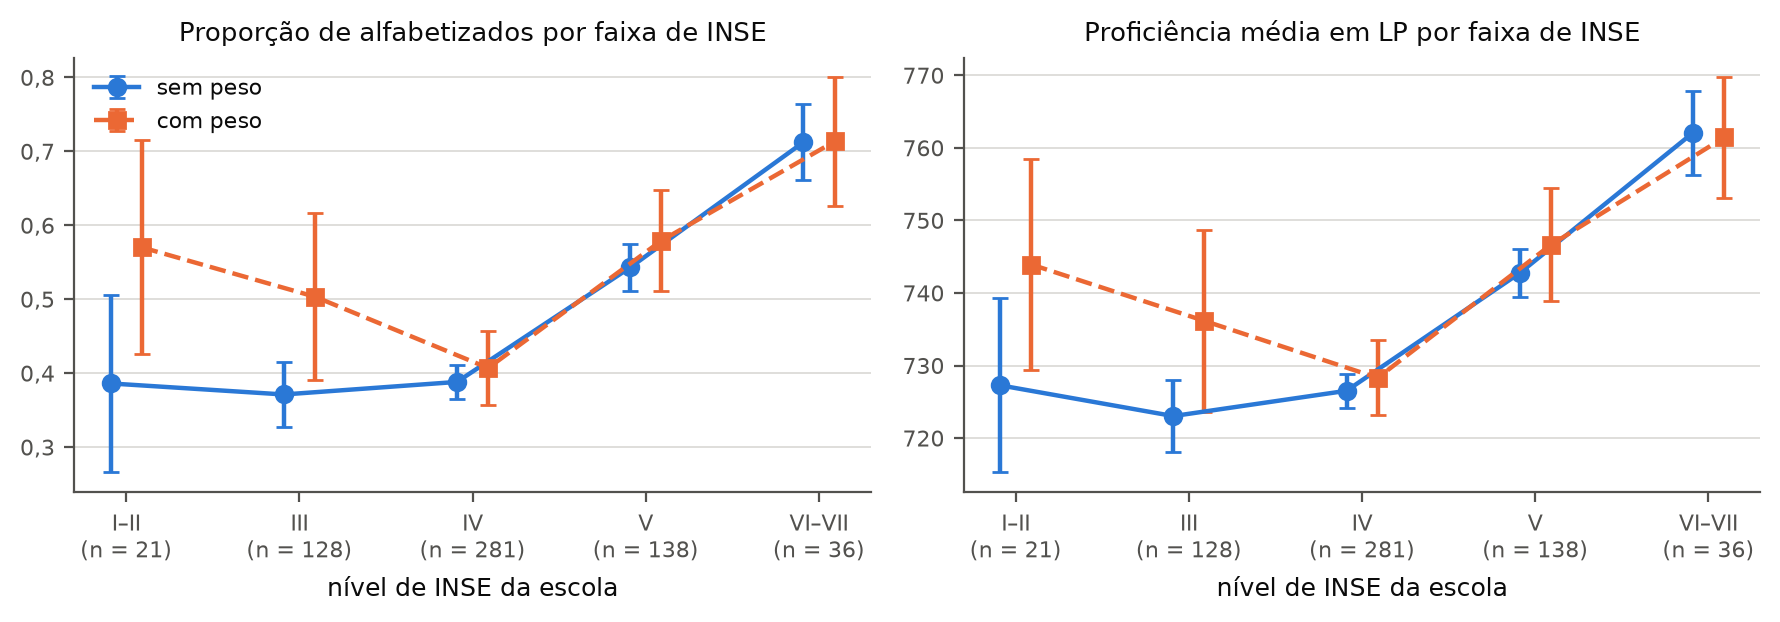
\includegraphics[width=\textwidth]{figuras/desfechos_por_inse.png}
    \begin{flushleft}
    {\footnotesize Fonte: elaborada pelo autor, com base nos microdados do
    Saeb 2023 (Inep). Barras: intervalo de confiança de 95\%. Com peso, o
    intervalo usa o tamanho efetivo de Kish.}
    \end{flushleft}
    \label{fig:desfechos-inse}
\end{figure}

Entre as regiões, a proporção sem peso vai de 37,5\% no Norte a 59,2\% no
Sul, que também tem o maior INSE médio (5,1, contra 3,8 no Norte). As
escolas rurais e as urbanas ficam próximas sem peso (42,1\% e 44,7\%).

As 54 escolas públicas excluídas por falta do INSE não diferem das
incluídas nos desfechos. A diferença média padronizada é de $-$0,02 na
proporção e de 0,03 na proficiência, com $p$ de 0,91 e 0,99 no teste de
Mann-Whitney. Também não diferem no porte, no número de turmas nem na
presença dos questionários. A diferença está na localização: 44,4\% das
excluídas são rurais, contra 29,1\% das incluídas (diferença padronizada de
$-$0,32, $p = 0{,}02$). A restrição ao INSE desloca a base para escolas
urbanas sem diferença detectável nos desfechos, e as execuções sem INSE da
Seção~\ref{sec:res-robustez} incluem as escolas excluídas.

A ausência de questionário é pouco informativa. As 85 escolas sem
questionário de professor têm proporção de alfabetizados de 40,0\%, contra
44,6\% das demais (diferença padronizada de 0,19, $p = 0{,}09$). Nas 28
escolas sem questionário de diretor, a proporção é de 37,7\%, contra 44,2\%
($p = 0{,}11$). As duas diferenças têm $p$ acima de 0,05 e apontam na mesma
direção, o que justifica manter os indicadores de não resposta entre os
preditores (Seção~\ref{sec:variaveis}).
